\begin{apendicesenv}

% ----------------------------------------------------------
\chapter{Conceitualização da OntoMPO}
\label{ap:conceitualizacao}
% ----------------------------------------------------------

\section{Glossário de termos}

\begin{table}[H]
\centering
\caption{Termos específicos da subcamada "Infraestrutura de TI" da camada "Estruturas".}
\begin{tabularx}{\textwidth}{|l|X|X|}
\hline
\textbf{Termo} & \textbf{Definição} & \textbf{Relações} \\ \hline
\textbf{Redes}   & Corresponde aos componentes (incluindo hardware e software) que possibilitam a comunicação, o gerenciamento e as operações de rede entre um observatório de projetos e os
sistemas internos e externos das organizações. & Suporta \textbf{Hardware}, \textbf{Serviços}, \textbf{Gerenciamento de dados} e \textbf{Software}.\\ \hline
\textbf{Hardware}   & Corresponde ao equipamento físico de tecnologia da informação utilizado nos processos executados pelos observatórios de projetos. & Suporta \textbf{Serviços}, \textbf{Gerenciamento de dados} e \textbf{Software}\\ \hline
\textbf{Serviços}   & Corresponde aos serviços executados por terceiros para estruturar, operar e manter a infraestrutura de TI de um observatório de projetos. & Suporta \textbf{Gerenciamento de dados} e \textbf{Software}.\\ \hline
\textbf{Gerenciamento de dados}   & Corresponde às ferramentas de software necessárias para que o observatório organize, gerencie e processe os dados relacionados aos projetos.
 & Viabiliza a \textbf{Coleta}, \textbf{Processamento} e \textbf{Armazenamento} dos dados. \\ \hline
\textbf{Software}  & Corresponde às aplicações que possibilitam a execução dos processos executados pelos observatórios de projetos. & Viabiliza a \textbf{Disseminação} e \textbf{Relacionamento} \\ \hline
\end{tabularx}
\end{table}

\begin{table}[H]
\centering
\caption{Termos específicos da subcamada "Características" da camada "Estruturas".}
\begin{tabularx}{\textwidth}{|l|X|X|}
\hline
\textbf{Termo} & \textbf{Definição} & \textbf{Relações} \\ \hline
\textbf{Sustentabilidade}   & Planejamento para o funcionamento do observatório no longo prazo. & Especifica estratégias de sustentabilidade para \textbf{Coleta}. \\ \hline
\textbf{Abragência} & Um observatório de projetos precisa ter seu escopo claramente definido. Nesse sentido,
esse escopo pode estar relacionado a: temática, região geográfica ou organização executora dos projetos contidos nos observatórios.
  & Especifica as estratégias de abragência da \textbf{Temática de Projetos}. \\ \hline
\textbf{Interoperabilidade} & Um observatório de projetos pode contemplar mecanismos que o tornem capaz de se comunicar de maneira transparente. & Especifica as estratégias de interoperabilidade para \textbf{Relacionamento}. \\ \hline
\textbf{Acesso} & Um observatório de projetos pode ser caracterizado como aberto ou semiaberto de acordo com seu escopo de visibilidade. & Especifica as políticas de acesso para \textbf{Disseminação} e \textbf{Relacionamento}. \\ \hline
\textbf{Rede de colaboração}   & Um observatório de projetos pode ser caracterizado como uma rede de colaboração, com um objetivo em comum: compartilhar dados, informações, e conhecimento sobre projetos. & Especifica as estratégias de rede de colaboração para o \textbf{Observatório}, \textbf{Projetos} e \textbf{Usuários}. \\ \hline
\textbf{Segurança}   & Devem ser implementadas medidas que garantam a segurança do observatório e dosdados contidos nele & Especifica as políticas de segurança para \textbf{Armazenamento}, \textbf{Disseminação} e \textbf{Relacionamento}. \\ \hline
\textbf{Interatividade}  & Um observatório de projetos pode permitir que haja interação entre os usuários e os projetos contidos no observatório. & Especifica as estratégias de interatividade dos \textbf{Usuários} com os \textbf{Projetos} e o \textbf{Observatório}. \\ \hline
\textbf{Formato dos dados} & Os dados armazenados podem ser estruturados ou não estruturados. & Especifica o formato de dados para \textbf{Processamento} e \textbf{Armazenamento}. \\ \hline
\textbf{Dados parciais}   & A existência de informações incompletas ou de caráter privado nos projetos exige que o observatório de projetos esteja preparado para armazenar dados parciais sobre esses projetos. & Especifica a completude dos dados para \textbf{Armazenamento}. \\ \hline
\end{tabularx}
\end{table}

\begin{table}[H]
\centering
\caption{Termos específicos da subcamada "Componentes" da camada "Estruturas".}
\begin{tabularx}{\textwidth}{|l|X|X|}
\hline
\textbf{Termo} & \textbf{Definição} & \textbf{Relações} \\ \hline
\textbf{Coleta} & Capturar de forma interna ou externa os dados dos projetos. & Coleta por meio da infraestrutura de \textbf{Gerenciamento de dados} de acordo com as estratégias de \textbf{Sustentabilidade}. \\ \hline
\textbf{Processamento} & Tratar e converter  os dados brutos relacionados aos projetos em uma forma mais significativa. & Obtem os dados, realiza o processamento por meio da infraestrutura de \textbf{Gerenciamento de dados} e adequa ao \textbf{Formato dos dados}. Considera-se pré-processamento quando a ação ocorre antes do \textbf{Armazenamento}, e pós-processamento quando ocorre após o \textbf{Armazenamento}.\\ \hline
\textbf{Armazenamento}  & Armazenar os dados relacionados aos projetos coletados pelos observatórios. & Armazena os dados, mantendo a referência aos dados brutos da \textbf{Coleta}, baseado nas diretrizes de \textbf{Segurança}, \textbf{Formato dos dados} e \textbf{Dados parciais} por meio da infraestrutura de \textbf{Gerenciamento de dados}.\\ \hline
\textbf{Disseminação}  & Divulgar análise e reflexões. & Divulga análises dos dados de \textbf{Projetos} por meio de um \textbf{Software} baseado nas diretrizes de \textbf{Acesso} e \textbf{Segurança}.\\ \hline
\textbf{Relacionamento}  & Coordenar os relacionamentos entre os \textbf{Usuários} e a interação desses com os projetos e o \textbf{Observatório}. Além disso, este conceito contempla os relacionamentos do observatório de projetos com outros sistemas. & Gerencia a interação entre usuários, sistemas externos e o observatório, utilizando o \textbf{Software} orientado pelas diretrizes de \textbf{Acesso}, \textbf{Segurança} e \textbf{Interoperabilidade}.\\ \hline
\end{tabularx}
\end{table}

\begin{table}[H]
\centering
\caption{Termos específicos da subcamada "Conteúdos" da camada "Estruturas".}
\begin{tabularx}{\textwidth}{|l|X|X|}
\hline
\textbf{Termo} & \textbf{Definição} & \textbf{Relações} \\ \hline
\textbf{Projetos}   & Um observatório poderá conter dados, informações e conhecimento relacionados aos projetos. & Especifica o conteúdo dos projetos do observatório para \textbf{Disseminação} baseado nas estratégias de \textbf{Interatividade} e \textbf{Rede de colaboração}.  \\ \hline
\textbf{Temáticas dos Projetos}  & Um observatório de projetos poderá ter conteúdo relacionado à temática dos projetos. & Especifica a temática dos \textbf{Projetos} baseado nas estratégias de \textbf{Abrangência}.\\ \hline
\textbf{Usuários}  & Os dados relacionados aos usuários e suas interações com o conteúdo do observatório de projetos também podem ser compreendidos como um conteúdo do observatório. & Especifica o conteúdo dos usuários do observatório para \textbf{Relacionamento} baseado nas estratégias de \textbf{Interatividade} e \textbf{Rede de colaboração}. \\ \hline
\textbf{Observatório}   & Informações gerais acerca do observatório também devem ser considerados conteúdo de um observatório de projetos. & Especifica o conteúdo do observatório para \textbf{Relacionamento} baseado nas estratégia de \textbf{Interatividade} e \textbf{Rede de colaboração}. \\ \hline
\end{tabularx}
\end{table}

\begin{table}[H]
\centering
\caption{Termos específicos da subcamada ``Gerenciar Dados e Informações`` da camada 
``Processos``.}
\begin{tabularx}{\textwidth}{|l|X|X|}
\hline
\textbf{Termo} & \textbf{Definição} & \textbf{Relações} \\ \hline
\textbf{Coletar}   & Corresponde a processos relacionados a identificação e coleta de dados e informações relevantes sobre os projetos e suas temáticas.  & Coleta manual ou automatizada por meio do componente de \textbf{Coleta}.\\ \hline
\textbf{Tratar}  & Corresponde a processos relacionados a organização e a garantia da qualidade e segurança dos dados e informações coletadas pelos observatórios de projetos. & Auditoria dos dados provenientes do processo \textbf{Coletar} por meio do componente \textbf{Processamento}. \\ \hline
\textbf{Armazenar}   & Corresponde aos processos de armazenamento, em um determinado repositório, dos dados e informações identificadas e coletadas pelo observatório de projetos.
 & Armazenamento automático por meio do componente de \textbf{Armazenamento}. \\ \hline
\textbf{Disponibilizar}   & Corresponde aos processos que possibilitam os usuários de um observatório de projetos acessarem os dados e informações coletadas antes de passarem por algum
processamento. & Disponibilização dos dados brutos coletados por meio do componente de \textbf{Armazenamento}. \\ \hline
\end{tabularx}
\end{table}

\begin{table}[H]
\centering
\caption{Termos específicos da subcamada "Produzir Conhecimento e Inteligência" da camada "Processos".}
\begin{tabularx}{\textwidth}{|l|X|X|}
\hline
\textbf{Termo} & \textbf{Definição} & \textbf{Relações} \\ \hline
\textbf{Transformar}   & Transformação e modelagem dos dados coletados pelo observatório de projetos.
 & Transformação dos dados por meio do componente de \textbf{Processamento}. \\ \hline
\textbf{Classificar}   & Identificar categorias e organizar relações entre os projetos. & Categorização dos dados por meio do componente de \textbf{Disseminação}. \\ \hline
\textbf{Comunicar}  & Comunicar para os
atores envolvidos com o observatório de projetos, todo o conteúdo do observatório, em
especial, as análises realizadas a partir dos dados coletados.
 & Compartilhamento dos dados por meio do componente de \textbf{Disseminação}. \\ \hline
\textbf{Visualizar}   & Construção de representações gráficas dos dados e informações. & Visualização dos dados de projetos por meio do componente de \textbf{Disseminação}. \\ \hline
\textbf{Combinar}   & Combinar diferentes fontes de dados e padrões relacionados aos projetos & Disponibilização do cruzamento de dados de projetos por meio do componente de \textbf{Disseminação}. \\ \hline
\textbf{Refletir}   &  Construção de reflexões críticas, por parte
dos atores do observatório de projetos, a partir dos dados e análises desenvolvidas acerca
dos projetos & Reflexões dos usuários sobre os projetos por meio do componente de \textbf{Disseminação}. \\ \hline
\textbf{Interagir}   & Permitem os atores de um observatório de projetos interagirem entre si e com o conteúdo do observatório. & Interação dos usuários com o observatório por meio do componente de \textbf{Relacionamento}. \\ \hline
\textbf{Acompanhar}   & Possibilitam os atores envolvidos com um observatório
de projetos acompanharem os projetos e sua evolução ao longo do tempo. & Acompanhamento dos projetos do observatório pelos usuários por meio do componente de \textbf{Relacionamento}. \\ \hline
\textbf{Avaliar}   &  Produzir avaliações sobre os projetos, sobre os
dados coletados e sobre as análises construídas a partir deles & Avaliação dos projetos pelos usuários por meio do componente de \textbf{Relacionamento}. \\ \hline
\textbf{Colaborar}   & Permitem os atores envolvidos com um observatório de projetos colaborarem com um projeto, caso desejarem. & Colaboração entre usuários e projetos do observatório por meio do componente de \textbf{Relacionamento}. \\ \hline
\textbf{Responsabilizar}   & Responsabilizar os atores do observatório de projetos por suas ações no contexto do observatório. & Auditoria das ações dos usuários no observatório por meio do componente de \textbf{Relacionamento}. \\ \hline
\end{tabularx}
\end{table}

\begin{table}[H]
\centering
\caption{Termos específicos da subcamada "Motivações" da camada "Agentes".}
\begin{tabularx}{\textwidth}{|l|X|X|}
\hline
\textbf{Termo} & \textbf{Definição} & \textbf{Relações} \\ \hline
\textbf{Transparência} & Buscam por mecanismos que possam oferecer transparência aos projetos. & Utilização dos processos \textbf{Comunicar}, \textbf{Visualizar}, \textbf{Combinar} e \textbf{Refletir} para o alcance das transparências em projetos. \\ \hline
\textbf{Conhecimento}  & Buscam adquirir e construir novos conhecimentos a partir do conteúdo disponibilizado pelo observatório de projetos.
 & Utilização dos processos \textbf{Comunicar}, \textbf{Visualizar}, \textbf{Combinar} e \textbf{Refletir} para viablizar conhecimento para os usuários. \\ \hline
\textbf{Tomada de decisão}  & Buscam por dados, informação e conhecimento para apoiar a tomada de decisão nos projetos. & Utilização dos processos \textbf{Comunicar}, \textbf{Visualizar}, \textbf{Combinar} e \textbf{Refletir} para auxiliar na tomada de decisão. \\ \hline
\textbf{Melhoria}   & Buscam por melhores práticas que proporcionem melhoria nos projetos e no seu gerenciamento. & Utilização dos processos \textbf{Comunicar}, \textbf{Visualizar}, \textbf{Combinar} e \textbf{Refletir} para identificar padrões e proporcionar melhorias nos projetos do observatório. \\ \hline
\textbf{Inovação}  & Buscam promover inovação nos projetos e nos produtos e serviços produzidos por eles,
por meio do conhecimento adquirido a partir de um observatório de projetos.
 & Utilização dos processos \textbf{Comunicar}, \textbf{Visualizar}, \textbf{Combinar} e \textbf{Refletir} para identificar possibilidade de inovação em projetos.\\ \hline
\textbf{Priorização} & Buscam por informações que auxiliem nos processos de priorização dos projetos.
 & Utilização do processo de \textbf{Categorização} para viabilizar o processo de priorização de projetos. \\ \hline
\textbf{Controle}  & Buscam por mecanismos que apoiem o controle sobre o planejamento e execução dos
projetos, proporcionando accountability aos projetos.
 & Utilização do processo \textbf{Acompanhar} para controlar e entender a evolução do projeto.\\ \hline
\textbf{Interação}   & Buscam por mecanismos que proporcionem interação entre as partes interessadas nos
projetos. & Utilização do processo \textbf{Interagir} para viabilizar a interação entre os usuários do observatório. \\ \hline
\textbf{Disseminação}  & Buscam disseminar boas e más experiências vividas nos projetos.
 & Utilização dos processos \textbf{Interagir} e \textbf{Colaborar} para troca de experiências entre os usuários do observatório. \\ \hline
\textbf{Aprendizagem} & Buscam aprender através da colaboração e do compartilhamento de dados, informação
e conhecimento sobre projetos. & Utilização dos processos \textbf{Interagir} e \textbf{Colaborar} para viabilizar a troca de conhecimento entre usuários do observatório. \\ \hline
\textbf{Engajamento}   & Buscam participação mais ativa das diversas partes interessadas no planejamento e
execução dos projetos.
 & Utilização dos processos \textbf{Interagir}, \textbf{Colaborar} e \textbf{Avaliar} para gerar engajamento nos projetos do observatório. \\ \hline
\end{tabularx}
\end{table}

\begin{table}[H]
\centering
\caption{Termos específicos da subcamada "Atores" da camada "Agentes".}
\begin{tabularx}{\textwidth}{|l|X|X|}
\hline
\textbf{Termo} & \textbf{Definição} & \textbf{Relações} \\ \hline
\textbf{Partes interessadas dos projetos}  & Uma parte interessada em um projeto pode ser compreendida
como um indivíduo, grupo ou organização que pode afetar ou ser afetada por uma
decisão, atividade ou resultado de um projeto. & Possuem as motivações de \textbf{Tomada de decisão}, \textbf{Melhoria} e \textbf{Inovação}. \\ \hline
\textbf{Equipe de gestão e desenvolvimento}  & Também podem ser considerados atores de um observatório de projetos, as equipes de gestão e de desenvolvimento do observatório. Compreendemos a equipe de gestão como o time responsável pelo gerenciamento, manutenção e operação do observatório. & Possuem as motivações de \textbf{Melhoria}, \textbf{Priorização} e \textbf{Controle}. \\ \hline
\textbf{Usuários do observatório} & Os usuários podem ser compreendidos como atores humanos que desfrutam das utilidades que um observatório de projetos proporciona. & Possuem as motivações de \textbf{Transparência}, \textbf{Conhecimento}, \textbf{Interação}, \textbf{Aprendizagem}, \textbf{Disseminação} e \textbf{Engajamento}.\\ \hline
\textbf{Sistemas}   & Os atores não-humanos, aqui chamados de sistemas, são representados pelos sistemas computacionais que não fazem parte do ambiente do observatório de projetos, no entanto, realizam alguma troca com o observatório, seja executando alguma ação ou
fornecendo algum serviço ao observatório.
 & Possui a motivação de transferência de \textbf{Conhecimento} entre sistemas. \\ \hline
\end{tabularx}
\end{table}

\section{Árvore de classificação de conceitos}

\begin{table}[H]
\centering
\caption{Conceitos específicos da subcamada "Infraestrutura de TI" da camada "Estruturas".}
\begin{tabularx}{\textwidth}{|l|X|X|X|X|}
\hline
\textbf{Conceito} & \textbf{Sinônimos} & \textbf{Descrição} & \textbf{Instâncias} \\ \hline
\textbf{Serviços}  & Prestação de serviços de TI e Outsorcing de TI. & Corresponde aos serviços executados por terceiros para estruturar, operar e manter a infraestrutura de TI de um observatório de projetos.& Hospedagem em nuvem e Hospedagem em servidor físico. \\ \hline
\textbf{Hardware}   & Equipamento de TI e dispositivo físico. & Corresponde ao equipamento físico de tecnologia da informação utilizado nos processos executados pelos observatórios de projetos. & Hardware de rede, processamento ou armazenamento. \\ \hline
\textbf{Redes}   & Infraestrutura de rede e Sistema de comunicação de dados. & Corresponde aos componentes (incluindo hardware e software) que possibilitam a comunicação, o gerenciamento e as operações de rede entre um observatório de projetos e os sistemas internos e externos das organizações. & Rede pública, rede privada, subrede ou VPN. \\ \hline
\textbf{Ger. de dados}   & Gestão de dados, Administração de dados e Data management.& Corresponde às ferramentas de software necessárias para que o observatório organize, gerencie e processe os dados relacionados aos projetos. & RDBMS, Data Warehouse, Data Lake ou Ferramenta de ETL. \\ \hline
\textbf{Software}  & Aplicações, Programas e Sistemas de informação & Corresponde às aplicações que possibilitam a execução dos processos executados pelos observatórios de projetos. & Trello, Jira, Teams ou Observatório. \\ \hline
\end{tabularx}
\end{table}

\begin{table}[H]
\centering
\caption{Atributos de classes do conceito "Serviços" da subcamada "Infraestrutura de TI" da camada "Estruturas".}
\begin{tabularx}{\textwidth}{|l|X|X|}
\hline
\textbf{Atributo} & \textbf{Descrição} \\ \hline
\textbf{Tipo}  & Define a categoria do serviço. \\ \hline
\textbf{Subtipo} & Área ou abrangência do serviço na infraestrutura de TI. \\ \hline
\end{tabularx}
\end{table}

\begin{table}[H]
\centering
\caption{Tabela de constantes do conceito "Serviços" da subcamada "Infraestrutura de TI" da camada "Estruturas".}
\begin{tabularx}{\textwidth}{|l|X|X|}
\hline
\textbf{Constante} & \textbf{Valores} \\ \hline
\textbf{Tipo}  & Suporte, Monitoramento, Segurança, Infraestrutura, Armazenamento, Integração ou Apresentação.  \\ \hline
\textbf{Subtipo} & Log, Rede, Banco de dados, Sistema de Arquivos, API, Terminal ou Interface gráfica.  \\ \hline
\end{tabularx}
\end{table}

\begin{table}[H]
\centering
\caption{Atributos de instâncias do conceito "Serviços" da subcamada "Infraestrutura de TI" da camada "Estruturas".}
\begin{tabularx}{\textwidth}{|l|X|X|}
\hline
\textbf{Atributo} & \textbf{Descrição} \\ \hline
\textbf{Provedor} & Indica quem presta o serviço (empresa, equipe terceirizada ou fornecedor). Exemplos: AWS, Microsoft ou empresa local de TI. \\ \hline
\textbf{Local} & Onde o serviço é efetivamente operado. Exemplo: Datacenter em São Paulo, nuvem pública AWS, nuvem privada local. \\ \hline
\textbf{Período} & Duração do contrato ou tempo em que o serviço é fornecido. Exemplo: 01/2024 a 12/2025. \\ \hline
\textbf{Custo} & Valor específico associado ao serviço contratado. Exemplo: 5.000,00 reais por mês para hospedagem. \\ \hline
\textbf{Disponibilidade} & Percentual ou indicador de tempo em que o serviço deve estar ativo. Exemplo: 99,9 uptime. \\ \hline
\end{tabularx}
\end{table}

\begin{table}[H]
\centering
\caption{Atributos de classes do conceito "Hardware" da subcamada "Infraestrutura de TI" da camada "Estruturas".}
\begin{tabularx}{\textwidth}{|l|X|X|}
\hline
\textbf{Atributo} & \textbf{Descrição} \\ \hline
\textbf{Tipo}  & Classificação do equipamento.\\ \hline
\textbf{Especificação} & Parâmetros gerais que definem a categoria do hardware. Exemplos: Arquitetura (x86, ARM), compatibilidade ou formato (rack, torre). \\ \hline
\textbf{Propósito} & Finalidade do hardware no ambiente de TI. Exemplos: Processar dados, Armazenar informações ou Interconectar redes. \\ \hline
\end{tabularx}
\end{table}

\begin{table}[H]
\centering
\caption{Tabelas de constantes do conceito "Hardware" da subcamada "Infraestrutura de TI" da camada "Estruturas".}
\begin{tabularx}{\textwidth}{|l|X|X|}
\hline
\textbf{Constante} & \textbf{Valores} \\ \hline
\textbf{Tipo}  & Servidor, Rede, Armazenamento, Processamento ou Vídeo. \\ \hline
\end{tabularx}
\end{table}

\begin{table}[H]
\centering
\caption{Atributos de instâncias do conceito "Hardware" da subcamada "Infraestrutura de TI" da camada "Estruturas".}
\begin{tabularx}{\textwidth}{|l|X|X|}
\hline
\textbf{Atributo} & \textbf{Descrição} \\ \hline
\textbf{Local} & Onde o equipamento está fisicamente localizado. Exemplos: Datacenter principal, sala de servidores ou estação de trabalho do usuário. \\ \hline
\textbf{Capacidade de processamento}  & Medida de desempenho do equipamento. Exemplos: 16 núcleos, 3.2 GHz ou 64 GB RAM. \\ \hline
\textbf{Capacidade de armazenamento} & Volume máximo de dados que o hardware pode guardar. Exemplos: 10 TB em disco rígido ou 2 TB em SSD. \\ \hline
\end{tabularx}
\end{table}

\begin{table}[H]
\centering
\caption{Atributos de classes do conceito "Redes" da subcamada "Infraestrutura de TI" da camada "Estruturas".}
\begin{tabularx}{\textwidth}{|l|X|X|}
\hline
\textbf{Atributo} & \textbf{Descrição} \\ \hline
\textbf{Tipo}  & Categoria que define a natureza da rede. \\ \hline
\textbf{Topologia} & Forma de organização física ou lógica. \\ \hline
\textbf{Abrangência} & Alcance organizacional ou geográfico. \\ \hline
\textbf{Protocolo} & Regras e padrões que suportam a comunicação. Exemplos: TCP/IP, UDP ou HTTP/HTTPS. \\ \hline
\end{tabularx}
\end{table}

\begin{table}[H]
\centering
\caption{Tabela de constantes do conceito "Redes" da subcamada "Infraestrutura de TI" da camada "Estruturas".}
\begin{tabularx}{\textwidth}{|l|X|X|}
\hline
\textbf{Constante} & \textbf{Valores} \\ \hline
\textbf{Tipo}  & Pública, Privada ou Híbrida. \\ \hline
\textbf{Topologia} & Barramento, Ponto a Ponto, Estrela, Anel, Árvore ou Híbrida. \\ \hline
\textbf{Abrangência} & LAN, MAN OU WAN. \\ \hline
\end{tabularx}
\end{table}

\begin{table}[H]
\centering
\caption{Atributos de instância do conceito "Redes" da subcamada "Infraestrutura de TI" da camada "Estruturas".}
\begin{tabularx}{\textwidth}{|l|X|X|}
\hline
\textbf{Atributo} & \textbf{Descrição} \\ \hline
\textbf{Local}  & Onde a rede é utilizada. Exemplos: Datacenter do observatório, nuvem pública ou rede de filial. \\ \hline
\textbf{Estado} & Situação atual da rede. Exemplos: Ativa, em manutenção ou desativada. \\ \hline
\textbf{Banda} & Capacidade máxima de transmissão de dados. Exemplos: 1 Gbps ou 10 Gbps. \\ \hline
\textbf{Segurança} & Grau de proteção implementado na rede. Exemplos: Alta (rede privada com firewall e criptografia), média ou baixa. \\ \hline
\end{tabularx}
\end{table}

\begin{table}[H]
\centering
\caption{Atributos de classe do conceito "Gerenciamento de dados" da subcamada "Infraestrutura de TI" da camada "Estruturas".}
\begin{tabularx}{\textwidth}{|l|X|X|}
\hline
\textbf{Atributo} & \textbf{Descrição} \\ \hline
\textbf{Tipo} & Classificação da solução de gerenciamento de dados. \\ \hline
\textbf{Modelo} & Modelo de implantação do serviço.\\ \hline
\textbf{Formato} & Estrutura de dados que a ferramenta manipula.\\ \hline
\textbf{Propósito} & Papel central da ferramenta no observatório. Exemplos: Armazenar dados, consolidar informações, transformar dados ou controlar acesso. \\ \hline
\end{tabularx}
\end{table}

\begin{table}[H]
\centering
\caption{Tabela de constantes do conceito "Gerenciamento de dados" da subcamada "Infraestrutura de TI" da camada "Estruturas".}
\begin{tabularx}{\textwidth}{|l|X|X|}
\hline
\textbf{Constante} & \textbf{Valores} \\ \hline
\textbf{Tipo} & Data warehouse, Data lake, Pipeline de dados, Integração de dados, Governança de dados, Catálogo de dados ou Orquestrador de dados.\\ \hline
\textbf{Modelo} & IaaS, PaaS ou SaaS. \\ \hline
\textbf{Formato} & Objeto, Grafo, Documento ou Multidimensional. \\ \hline
\end{tabularx}
\end{table}

\begin{table}[H]
\centering
\caption{Atributos de instância do conceito "Gerenciamento de dados" da subcamada "Infraestrutura de TI" da camada "Estruturas".}
\begin{tabularx}{\textwidth}{|l|X|X|}
\hline
\textbf{Atributo} & \textbf{Descrição} \\ \hline
\textbf{Nome} & Identificação específica da ferramenta. Exemplos: PostgreSQL, MySQL, MongoDB ou SQLServer. \\ \hline
\textbf{Versão} & Versão do software instalada. Exemplos: PostgreSQL 16.1 ou Oracle 21c. \\ \hline
\end{tabularx}
\end{table}

\begin{table}[H]
\centering
\caption{Atributos de classe do conceito "Software" da subcamada "Infraestrutura de TI" da camada "Estruturas".}
\begin{tabularx}{\textwidth}{|l|X|X|}
\hline
\textbf{Atributo} & \textbf{Descrição} \\ \hline
\textbf{Modelo} & Modelo de implantação do serviço. \\ \hline
\textbf{Ambiente} & Ambiente em que o software funciona. \\ \hline
\textbf{Licenciamento} & Forma de disponibilização e uso. \\ \hline
\textbf{Propósito} & Papel central da ferramenta no observatório. Exemplos: Gerenciamento de atividades, comunicação ou da própria aplicação. \\ \hline
\end{tabularx}
\end{table}

\begin{table}[H]
\centering
\caption{Tabela de constantes do conceito "Software" da subcamada "Infraestrutura de TI" da camada "Estruturas".}
\begin{tabularx}{\textwidth}{|l|X|X|}
\hline
\textbf{Constante} & \textbf{Valores} \\ \hline
\textbf{Modelo} & IaaS, PaaS ou SaaS. \\ \hline
\textbf{Ambiente} & Web, Desktop ou Mobile.\\ \hline
\textbf{Licenciamento} & Aberto, Proprietário ou Híbrido.\\ \hline
\end{tabularx}
\end{table}

\begin{table}[H]
\centering
\caption{Atributos de instância do conceito "Software" da subcamada "Infraestrutura de TI" da camada "Estruturas".}
\begin{tabularx}{\textwidth}{|l|X|X|}
\hline
\textbf{Atributo} & \textbf{Descrição} \\ \hline
\textbf{Nome} & Identificação específica da aplicação. Ex.: Trello, Jira, Teams ou Observatório. \\ \hline
\textbf{Versão} & Lançamento ou release em uso. Exemplos: v1.0.0-rc ou v2.0.0. \\ \hline
\end{tabularx}
\end{table}


\begin{table}[H]
\centering
\caption{Conceitos específicos da subcamada "Componentes" da camada "Estruturas".}
\begin{tabularx}{\textwidth}{|l|X|X|X|X|}
\hline
\textbf{Conceito} & \textbf{Sinônimos} & \textbf{Descrição} & \textbf{Instâncias} \\ \hline
\textbf{Coleta} & Captura de dados, aquisição de dados e data collection. & Capturar de forma interna ou externa os dados dos projetos. & Coleta manual, automática, via questionários, por integração de sistemas ou por sensores/IoT\\ \hline
\textbf{Processamento} & Tratamento de dados, transformação de dados e data processing. & Tratar e converter os dados brutos relacionados aos projetos em uma forma mais significativa. & Batch, streaming, processamento estatístico, analítico ou por machine learning.\\ \hline
\textbf{Armazenamento}  & Repositório de dados, memória de dados ou data storage & Armazenar os dados relacionados aos projetos coletados pelos observatórios. & Relacional, não relacional, data warehouse, data lake, sistema de arquivos distribuído ou armazenamento em nuvem. \\ \hline
\textbf{Disseminação}  & Divulgação, comunicação e publicação de resultados. & Divulgar análises e reflexões produzidas pelo observatório de projetos. & Relatórios técnicos, dashboards interativos, artigos científicos, newsletters ou apresentações institucionais.\\ \hline
\textbf{Relacionamento} & Interação, vinculação e conexão & Coordenar os relacionamentos entre os usuários e a interação desses com os projetos e o observatório. Além disso, este conceito contempla os relacionamentos do observatório de projetos com outros sistemas. & Relacionamento usuário–projeto, usuário–observatório, observatório–sistemas externos. \\ \hline
\end{tabularx}
\end{table}

\begin{table}[H]
\centering
\caption{Atributos de classe do conceito "Coleta" da subcamada "Componentes" da camada "Estruturas".}
\begin{tabularx}{\textwidth}{|l|X|X|}
\hline
\textbf{Atributo} & \textbf{Descrição} \\ \hline
\textbf{Método} & Forma como os dados são obtidos.\\ \hline
\textbf{Fonte} & Origem principal dos dados coletados. Exemplos: Sistemas internos, stakeholders externos, bases de dados abertas ou sensores.\\ \hline
\textbf{Frequência} & Periodicidade prevista para a captura. Exemplos: Contínua, diária, semanal ou sob demanda. \\ \hline
\end{tabularx}
\end{table}

\begin{table}[H]
\centering
\caption{Tabela de constantes do conceito "Coleta" da subcamada "Componentes" da camada "Estruturas".}
\begin{tabularx}{\textwidth}{|l|X|X|}
\hline
\textbf{Constante} & \textbf{Valores} \\ \hline
\textbf{Método} & Manual, Automática ou Híbrida. \\ \hline
\end{tabularx}
\end{table}

\begin{table}[H]
\centering
\caption{Atributos de instância do conceito "Coleta" da subcamada "Componentes" da camada "Estruturas".}
\begin{tabularx}{\textwidth}{|l|X|X|}
\hline
\textbf{Atributo} & \textbf{Descrição} \\ \hline
\textbf{Ferramenta} & Software ou recurso aplicado na coleta. Exemplos: Google Forms, ETL Talend, API REST, planilha Excel. \\ \hline
\textbf{Volume} & Quantidade registrada em uma sessão de coleta. Exemplos: 200 registros ou 5GB  de dados. \\ \hline
\textbf{Qualidade} & Avaliação da completude, consistência e precisão dos dados coletados. Exemplos: Alta, média ou baixa.\\ \hline
\end{tabularx}
\end{table}

\begin{table}[H]
\centering
\caption{Atributos de classe do conceito "Processamento" da subcamada "Componentes" da camada "Estruturas".}
\begin{tabularx}{\textwidth}{|l|X|X|}
\hline
\textbf{Atributo} & \textbf{Descrição} \\ \hline
\textbf{Método} & Forma pela qual os dados são processados.\\ \hline
\textbf{Escopo} & Conjunto de dados abrangido. Exemplos: Todos os projetos, subconjunto de projetos, dados históricos ou dados em fluxo.  \\ \hline
\textbf{Nível de automação} & Grau de intervenção humana no processo de processamento. \\ \hline
\textbf{Propósito} & Objetivo central da transformação de dados. Exemplos: Limpeza, enriquecimento, agregação ou análise preditiva. \\ \hline
\end{tabularx}
\end{table}

\begin{table}[H]
\centering
\caption{Tabela de constantes do conceito "Processamento" da subcamada "Componentes" da camada "Estruturas".}
\begin{tabularx}{\textwidth}{|l|X|X|}
\hline
\textbf{Constante} & \textbf{Valores} \\ \hline
\textbf{Método} & Batch, Síncrono, Assíncrono ou Híbrido. \\ \hline
\textbf{Nível de automação} & Manual, Automático ou Híbrido. \\ \hline
\end{tabularx}
\end{table}

\begin{table}[H]
\centering
\caption{Atributos de instância do conceito "Processamento" da subcamada "Componentes" da camada "Estruturas".}
\begin{tabularx}{\textwidth}{|l|X|X|}
\hline
\textbf{Atributo} & \textbf{Descrição} \\ \hline
\textbf{Ferramenta} & Software ou recurso empregado. Exemplos: Python (Pandas), R, Apache Spark ou Power BI Dataflows.\\ \hline
\textbf{Volume} & Quantidade de dados processados em uma execução. Exemplos: 50 mil registros ou 30 GB de dados.\\ \hline
\textbf{Desempenho} & Tempo ou eficiência da execução do processamento. Exemplos: 5 segundos, 2 horas ou processamento distribuído. \\ \hline
\textbf{Resultado} & Saída concreta do processamento. Exemplos: Relatório, dataset consolidado ou modelo preditivo. \\ \hline
\end{tabularx}
\end{table}

\begin{table}[H]
\centering
\caption{Atributos de classe do conceito "Armazenamento" da subcamada "Componentes" da camada "Estruturas".}
\begin{tabularx}{\textwidth}{|l|X|X|}
\hline
\textbf{Atributo} & \textbf{Descrição} \\ \hline
\textbf{Tipo}& Categoria do recurso. \\ \hline
\textbf{Modelo}& Estrutura utilizada para guardar informações.\\ \hline
\textbf{Durabilidade}& Forma de retenção dos dados ao longo do tempo. Exemplos: Temporário ou permanente.\\ \hline
\textbf{Propósito}& Propósito principal da solução. Exemplos: Transacional (OLTP), analítico (OLAP), histórico ou backup. \\ \hline
\end{tabularx}
\end{table}

\begin{table}[H]
\centering
\caption{Tabela de constantes do conceito "Armazenamento" da subcamada "Componentes" da camada "Estruturas".}
\begin{tabularx}{\textwidth}{|l|X|X|}
\hline
\textbf{Constante} & \textbf{Valores} \\ \hline
\textbf{Tipo} & Banco de dados ou Sistema de arquivos. \\ \hline
\textbf{Modelo}& Relacional, Documentos, Grafos, Chave-valor ou Objeto. \\ \hline
\end{tabularx}
\end{table}

\begin{table}[H]
\centering
\caption{Atributos de instância do conceito "Armazenamento" da subcamada "Componentes" da camada "Estruturas".}
\begin{tabularx}{\textwidth}{|l|X|X|}
\hline
\textbf{Atributo} & \textbf{Descrição} \\ \hline
\textbf{Local}& Onde os dados são efetivamente guardados. Exemplos: Datacenter local, nuvem pública ou nuvem privada. \\ \hline
\textbf{Capacidade}& Quantidade máxima de dados suportada. Exemplos: 5 TB, 100 TB ou sob demanda.\\ \hline
\end{tabularx}
\end{table}

\begin{table}[H]
\centering
\caption{Atributos de classe do conceito "Disseminação" da subcamada "Componentes" da camada "Estruturas".}
\begin{tabularx}{\textwidth}{|l|X|X|}
\hline
\textbf{Atributo} & \textbf{Descrição} \\ \hline
\textbf{Público-alvo} & Grupo a quem se destina a informação. Exemplos: Gestores de projetos, comunidade científica ou sociedade cívil.\\ \hline
\textbf{Propósito} & Objetivo principal da divulgação. Exemplos: Tomada de decisão, prestação de contas ou compartilhamento de conhecimento. \\ \hline
\end{tabularx}
\end{table}

\begin{table}[H]
\centering
\caption{Atributos de instância do conceito "Disseminação" da subcamada "Componentes" da camada "Estruturas".}
\begin{tabularx}{\textwidth}{|l|X|X|}
\hline
\textbf{Atributo} & \textbf{Descrição} \\ \hline
\textbf{Canal} & Meio pelo qual a informação é divulgada. Exemplos: Relatório, portal web, evento ou e-mail. \\ \hline
\textbf{Frequência} & Periodicidade prevista para a disseminação. Exemplos: Contínua, mensal, trimestral ou sob demanda. \\ \hline
\textbf{Ferramenta} & Aplicativo ou plataforma que suporta a divulgação. Exemplos: Portal web, Power BI, Tableau, LaTeX, WordPress, YouTube. \\ \hline
\textbf{Formato}  & Forma do conteúdo disseminado. Exemplos: Página web, Json, CSV, Excel, PDF ou vídeo. \\ \hline
\textbf{Alcance} & Medida de impacto ou número de destinatários atingidos. Exemplos: 100 gestores de projetos ou 500 visualizações em dashboard. \\ \hline
\end{tabularx}
\end{table}

\begin{table}[H]
\centering
\caption{Atributos de classe do conceito "Relacionamento" da subcamada "Componentes" da camada "Estruturas".}
\begin{tabularx}{\textwidth}{|l|X|X|}
\hline
\textbf{Atributo} & \textbf{Descrição} \\ \hline
\textbf{Tipo} & Categoria do vínculo estabelecido. \\ \hline
\textbf{Propósito} & Propósito principal da interação. Exemplos: Gestão de projetos, compartilhamento de informações ou integração de sistemas. \\ \hline
\end{tabularx}
\end{table}

\begin{table}[H]
\centering
\caption{Tabela de constantes do conceito "Relacionamento" da subcamada "Componentes" da camada "Estruturas".}
\begin{tabularx}{\textwidth}{|l|X|X|}
\hline
\textbf{Constante} & \textbf{Valores} \\ \hline
\textbf{Relacionamento} & Humano-Sistema ou Sistema-Sistema. \\ \hline
\end{tabularx}
\end{table}

\begin{table}[H]
\centering
\caption{Atributos de instância do conceito "Relacionamento" da subcamada "Componentes" da camada "Estruturas".}
\begin{tabularx}{\textwidth}{|l|X|X|}
\hline
\textbf{Atributo} & \textbf{Descrição} \\ \hline
\textbf{Canal} & Meio pelo qual ocorre a interação. Exemplos: E-mail, plataforma web, API de integração ou reunião presencial. \\ \hline
\textbf{Frequência} & Periodicidade do contato ou troca de informações. Exemplos: Diária, semanal, mensal, sob demanda. \\ \hline
\end{tabularx}
\end{table}

\begin{table}[H]
\centering
\caption{Conceitos específicos da subcamada "Conteúdos" da camada "Estruturas".}
\begin{tabularx}{\textwidth}{|l|X|X|X|X|}
\hline
\textbf{Conceito} & \textbf{Sinônimos} & \textbf{Descrição} & \textbf{Instâncias} \\ \hline
\textbf{Projetos}   & Empreendimentos, iniciativas e ações organizacionais. & Um observatório poderá conter dados, informações e conhecimento relacionados aos projetos. & Projeto de pesquisa, inovação, capacitação, infraestrutura ou desenvolvimento de software  \\ \hline
\textbf{Usuários}  & Participantes, agentes e atores do observatório. & Os dados relacionados aos usuários e suas interações com o conteúdo do observatório de projetos também podem ser compreendidos como um conteúdo do observatório. & Gestor de projetos, analista de dados ou desenvolvedor. \\ \hline
\textbf{Observatório}   & Centro de monitoramento de projetos, plataforma de acompanhamento de projetos e núcleo de gestão de projetos. & Informações gerais acerca do observatório também devem ser consideradas conteúdo de um observatório de projetos. & Observatório de Projetos de TI, pesquisa ou institucionais \\ \hline
\end{tabularx}
\end{table}

\begin{table}[H]
\centering
\caption{Atributos de classe do conceito "Projetos" da subcamada "Conteúdos" da camada "Estruturas".}
\begin{tabularx}{\textwidth}{|l|X|X|}
\hline
\textbf{Atributo} & \textbf{Descrição} \\ \hline
\textbf{Tipo} & Classificação do projeto. Exemplos: Pesquisa, inovação, capacitação, infraestrutura ou desenvolvimento de software. \\ \hline
\textbf{Temática} & Campo ou domínio a que o projeto pertence. Exemplos: Tecnologia da informação, saúde, educação ou engenharia. \\ \hline
\textbf{Objetivo} & Finalidade central do projeto. Exemplos: Desenvolver um sistema, formar profissionais ou gerar novo conhecimento. \\ \hline
\textbf{Escopo} & Limites ou abrangência do projeto.\\ \hline
\end{tabularx}
\end{table}

\begin{table}[H]
\centering
\caption{Tabela de constantes do conceito "Projetos" da subcamada "Conteúdos" da camada "Estruturas".}
\begin{tabularx}{\textwidth}{|l|X|X|}
\hline
\textbf{Constante} & \textbf{Valores} \\ \hline
\textbf{Escopo} & Institucional, Regional, Nacional ou Internacional.\\ \hline
\end{tabularx}
\end{table}

\begin{table}[H]
\centering
\caption{Atributos de instância do conceito "Projetos" da subcamada "Conteúdos" da camada "Estruturas".}
\begin{tabularx}{\textwidth}{|l|X|X|}
\hline
\textbf{Atributo} & \textbf{Descrição} \\ \hline
\textbf{Nome} & Identificação específica do projeto. Exemplos: Sistema Integrado de Gestão de Projetos. \\ \hline
\textbf{Duração} & Prazo de duração do projeto. Exemplos: 2024 até 2025 ou 01/2025 até 06/2025. \\ \hline
\textbf{Orçamento} & Recursos financeiros destinados ao projeto. Exemplos: Sem custos ou 50.000 reais. \\ \hline
\textbf{Descrição} & Detalhes sobre o projeto. Exemplos: O sistema visa aumentar a visibilidade dos projetos da Universidade de Pernambuco ou estimular o compartilhamento de conhecimento entre projetos. \\ \hline
\textbf{Responsável} & Grupo encarregado da execução. Exemplos: equipe de TI, equipe de pesquisa ou consultoria externa. \\ \hline
\textbf{Status} & Situação atual do projeto. Exemplos: Em planejamento, em execução, concluído o cancelado. \\ \hline
\end{tabularx}
\end{table}

\begin{table}[H]
\centering
\caption{Atributos de classe do conceito "Usuários" da subcamada "Conteúdos" da camada "Estruturas".}
\begin{tabularx}{\textwidth}{|l|X|X|}
\hline
\textbf{Atributo} & \textbf{Descrição} \\ \hline
\textbf{Propósito} & Função desempenhada pelo usuário. Exemplos: Coordenar projetos, analisar dados ou alimentar informações. \\ \hline
\end{tabularx}
\end{table}

\begin{table}[H]
\centering
\caption{Atributos de instância do conceito "Usuários" da subcamada "Conteúdos" da camada "Estruturas".}
\begin{tabularx}{\textwidth}{|l|X|X|}
\hline
\textbf{Atributo} & \textbf{Descrição} \\ \hline
\textbf{Ação} & Registro das atividades do usuário no observatório. Exemplos: Acessos, consultas realizadas ou atualizações feitas. \\ \hline
\end{tabularx}
\end{table}

\begin{table}[H]
\centering
\caption{Atributos de classe do conceito "Observatório" da subcamada "Conteúdos" da camada "Estruturas".}
\begin{tabularx}{\textwidth}{|l|X|X|}
\hline
\textbf{Atributo} & \textbf{Descrição} \\ \hline
\textbf{Tema} & Campo temático de aplicação. Exemplos: Tecnologia da informação, saúde ou educação. \\ \hline
\textbf{Propósito} & Propósito principal. Exemplos: Monitorar, analisar ou disseminar informações sobre projetos. \\ \hline
\textbf{Escopo} & Nível de abrangência.\\ \hline
\end{tabularx}
\end{table}

\begin{table}[H]
\centering
\caption{Tabela de constantes do conceito "Observatório" da subcamada "Conteúdos" da camada "Estruturas".}
\begin{tabularx}{\textwidth}{|l|X|X|}
\hline
\textbf{Constante} & \textbf{Valores} \\ \hline
\textbf{Escopo} & Nível de abrangência. Exemplos: Institucional, regional, nacional ou internacional. \\ \hline
\end{tabularx}
\end{table}

\begin{table}[H]
\centering
\caption{Atributos de instância do conceito "Observatório" da subcamada "Conteúdos" da camada "Estruturas".}
\begin{tabularx}{\textwidth}{|l|X|X|}
\hline
\textbf{Atributo} & \textbf{Descrição} \\ \hline
\textbf{Nome} & Identificação oficial. Exemplos: Observatório Nacional de Projetos de Inovação ou Observatório de Projetos da Universidade de Pernambuco. \\ \hline
\textbf{Instituição} & Organização que mantém o observatório. Exemplos: Universidade Federal, Ministério da Educação ou Secretaria de TI. \\ \hline
\end{tabularx}
\end{table}

\begin{figure}[H]
    \centering
    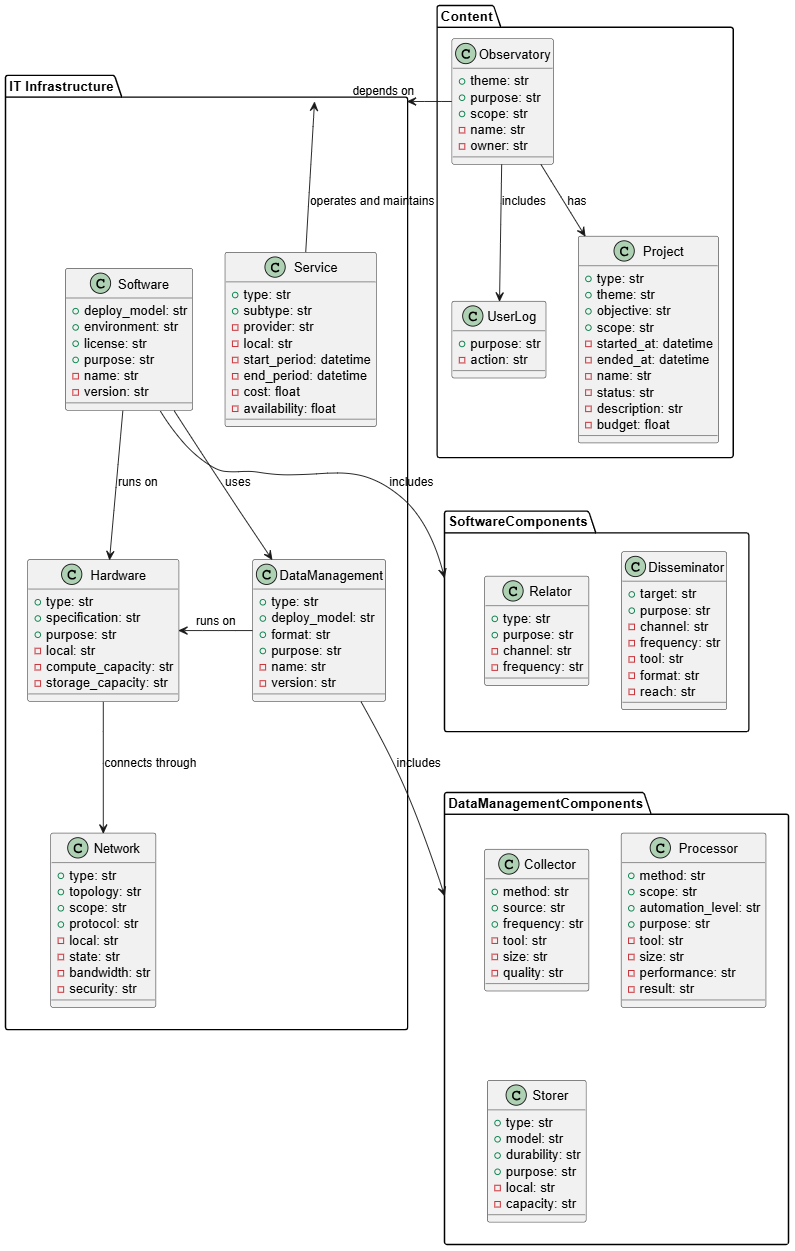
\includegraphics[width=1\linewidth]{imagens/mpo_structures_classification_tree.png}
    \caption{Árvore de classificação de conceitos da camada estruturas do MPO}
    \label{fig:mpo_class_tree}
\end{figure}

\begin{table}[H]
\centering
\caption{Termos específicos da subcamada "Atores" da camada "Agentes".}
\begin{tabularx}{\textwidth}{|l|X|X|X|X|}
\hline
\textbf{Conceito} & \textbf{Sinônimos} & \textbf{Descrição} & \textbf{Instâncias} \\ \hline
\textbf{Partes interessadas}  & Partes interessadas, Envolvidos e Atores externos/internos & Um indivíduo, grupo ou organização que pode afetar ou ser afetada por uma decisão, atividade ou resultado de um projeto. & Cliente, Patrocinador ou Grupo de pesquisa.  \\ \hline
\textbf{Equipe do obs.}  & Time do observatório, Grupo de gestão e Corpo técnico do observatório & Time responsável pelo gerenciamento, manutenção e operação do observatório. & Equipe de gestão, desenvolvimento ou suporte técnico.  \\ \hline
\textbf{Usuários do obs.} & Atores humanos, utilizadores e participantes. & Usuários que desfrutam das funcionalidades do observatório. & Gestores de projetos, analistas de dados, pesquisadores ou estudantes.  \\ \hline
\textbf{Sistemas}   & Sistemas externos, integrados e aplicações não pertencentes ao observatório. & Os atores não humanos, aqui chamados de sistemas, são representados pelos sistemas computacionais que não fazem parte do ambiente do observatório de projetos, mas realizam alguma troca com o observatório, seja executando alguma ação ou fornecendo algum serviço. & Sistema de gestão institucional, gestão de projetos, informação geográfica, SRH, plataforma de dados abertos ou API pública de indicadores.\\ \hline
\end{tabularx}
\end{table}

\begin{table}[H]
\centering
\caption{Atributos de classe do conceito "Partes interessadas" da subcamada "Atores" da camada "Agentes".}
\begin{tabularx}{\textwidth}{|l|X|X|}
\hline
\textbf{Atributo} & \textbf{Descrição} \\ \hline
\textbf{Tipo} & Categoria da parte interessada.\\ \hline
\textbf{Perfil} & Função desempenhada no contexto do projeto. Exemplos: Financiador, executor, beneficiário ou regulador.\\ \hline
\textbf{Grau de influência} & Capacidade de impactar decisões ou resultados do projeto.\\ \hline
\textbf{Nível de interesse} & Intensidade do envolvimento com os resultados do projeto. Exemplos: Alto (patrocinador), médio (usuários finais) ou baixo (público indireto). \\ \hline
\end{tabularx}
\end{table}

\begin{table}[H]
\centering
\caption{Tabela de constantes do conceito "Partes interessadas" da subcamada "Atores" da camada "Agentes".}
\begin{tabularx}{\textwidth}{|l|X|X|}
\hline
\textbf{Constante} & \textbf{Valores} \\ \hline
\textbf{Tipo} & Interno ou Externo. \\ \hline
\textbf{Grau de influência} & Alta, Média ou Baixa.\\ \hline
\textbf{Nível de interesse} & Alto, Médio ou Baixo. \\ \hline
\end{tabularx}
\end{table}

\begin{table}[H]
\centering
\caption{Atributos de instância do conceito "Partes interessadas" da subcamada "Atores" da camada "Agentes".}
\begin{tabularx}{\textwidth}{|l|X|X|}
\hline
\textbf{Atributo} & \textbf{Descrição} \\ \hline
\textbf{Nome} & Identificação da parte interessada. Exemplos: João, departamento de TI ou secretaria de ciência e tecnologia. \\ \hline
\textbf{Organização} & Instituição ao qual o stakeholder pertence. Exemplos: UPE, ministério da educação ou prefeitura.  \\ \hline
\textbf{Contato} & Informação de comunicação. Exemplos: E-mail, telefone ou endereço institucional.\\ \hline
\end{tabularx}
\end{table}

\begin{table}[H]
\centering
\caption{Atributos de classe do conceito "Equipe do observatório" da subcamada "Atores" da camada "Agentes".}
\begin{tabularx}{\textwidth}{|l|X|X|}
\hline
\textbf{Atributo} & \textbf{Descrição} \\ \hline
\textbf{Tipo} & Categoria da equipe dentro do observatório. \\ \hline
\textbf{Propósito} & Papel central da equipe no funcionamento do observatório. Exemplos: Gerenciar, desenvolver, manter ou apoiar decisões estratégicas. \\ \hline
\end{tabularx}
\end{table}

\begin{table}[H]
\centering
\caption{Tabela de constantes do conceito "Equipe do observatório" da subcamada "Atores" da camada "Agentes".}
\begin{tabularx}{\textwidth}{|l|X|X|}
\hline
\textbf{Constante} & \textbf{Valores} \\ \hline
\textbf{Tipo} & Administrativo, Financeiro, RH, Gestão, Desenvolvimento ou Suporte. \\ \hline
\end{tabularx}
\end{table}

\begin{table}[H]
\centering
\caption{Atributos de instância do conceito "Equipe do observatório" da subcamada "Atores" da camada "Agentes".}
\begin{tabularx}{\textwidth}{|l|X|X|}
\hline
\textbf{Atributo} & \textbf{Descrição} \\ \hline
\textbf{Nome} & Identificação formal. Exemplos: Equipe de gestão de projetos ou desenvolvimento. \\ \hline
\textbf{Membros} & Lista de integrantes da equipe. \\ \hline
\textbf{Responsável} & Pessoa que lidera ou coordena a equipe. Exemplos: Coordenador do observatório ou gerente de TI. \\ \hline
\end{tabularx}
\end{table}

\begin{table}[H]
\centering
\caption{Atributos de classe do conceito "Usuários do observatório" da subcamada "Atores" da camada "Agentes".}
\begin{tabularx}{\textwidth}{|l|X|X|}
\hline
\textbf{Atributo} & \textbf{Descrição} \\ \hline
\textbf{Tipo} & Categoria do ator humano que interage com o observatório. Exemplos: Gestor, analista, pesquisador, estudante ou cidadão externo. \\ \hline
\textbf{Perfil} & Nível de permissão ou privilégio concedido. Exemplos: Administrador, editor ou leitor. \\ \hline
\textbf{Propósito} & Objetivo principal da utilização. Exemplos: Consulta de informações, análise de dados, acompanhamento de projetos ou tomada de decisão. \\ \hline
\end{tabularx}
\end{table}

\begin{table}[H]
\centering
\caption{Atributos de instância do conceito "Usuários do observatório" da subcamada "Atores" da camada "Agentes".}
\begin{tabularx}{\textwidth}{|l|X|X|}
\hline
\textbf{Atributo} & \textbf{Descrição} \\ \hline
\textbf{Nome} & Identificação nominal. \\ \hline
\textbf{Organização} & Organização à qual o usuário pertence. Exemplos: Universidade de Pernambuco, prefeitura de Recife ou secretaria de saúde. \\ \hline
\textbf{Status} & Situação atual do usuário. Exemplos: Ativo, inativo ou bloqueado. \\ \hline
\end{tabularx}
\end{table}

\begin{table}[H]
\centering
\caption{Atributos de classe do conceito "Sistemas" da subcamada "Atores" da camada "Agentes".}
\begin{tabularx}{\textwidth}{|l|X|X|}
\hline
\textbf{Atributo} & \textbf{Descrição} \\ \hline
\textbf{Tipo} & Categoria do sistema externo.\\ \hline
\textbf{Propósito} & Propósito da troca de informações com o observatório. Exemplos: Fornecer dados, autenticar usuários ou disponibilizar relatórios. \\ \hline
\textbf{Método de comunicação} & Forma como ocorre a interação técnica entre os sistemas.\\ \hline
\textbf{Nível de interoperabilidade} & Grau de compatibilidade e automação da integração. \\ \hline
\end{tabularx}
\end{table}

\begin{table}[H]
\centering
\caption{Tabela de constantes do conceito "Sistemas" da subcamada "Atores" da camada "Agentes".}
\begin{tabularx}{\textwidth}{|l|X|X|}
\hline
\textbf{Constante} & \textbf{Valores} \\ \hline
\textbf{Tipo} & Governamental, Corporativo, Acadêmico ou Público \\ \hline
\textbf{Método de comunicação} & API, WebService ou Importação/Exportação de arquivos. \\ \hline
\textbf{Nível de interoperabilidade} & Manual, Automático ou Híbrido. \\ \hline
\end{tabularx}
\end{table}

\begin{table}[H]
\centering
\caption{Atributos de instância do conceito "Sistemas" da subcamada "Atores" da camada "Agentes".}
\begin{tabularx}{\textwidth}{|l|X|X|}
\hline
\textbf{Atributo} & \textbf{Descrição} \\ \hline
\textbf{Nome} & Identificação oficial. Exemplos: Sig@, SEI, Lattes ou dados do governo. \\ \hline
\textbf{Organização} & Organização mantenedora do sistema. Exemplos: Ministério da Educação, CNPq, Prefeitura Municipal. \\ \hline
\textbf{Tecnologia} & Base tecnológica ou linguagem predominante. Ex.: Java, .NET ou Python. \\ \hline
\textbf{Tipo de dado trocado} & Natureza da informação compartilhada. Exemplos: Dados de projetos, indicadores de desempenho ou metadados cadastrais. \\ \hline
\textbf{Frequência de integração} & Periodicidade da troca de dados. Exemplos: Em tempo real, diária, semanal ou sob demanda. \\ \hline
\textbf{Status de conexão} & Situação atual da integração. Exemplos: Ativa, em teste, suspensa ou encerrada. \\ \hline
\end{tabularx}
\end{table}

\begin{figure}[H]
    \centering
    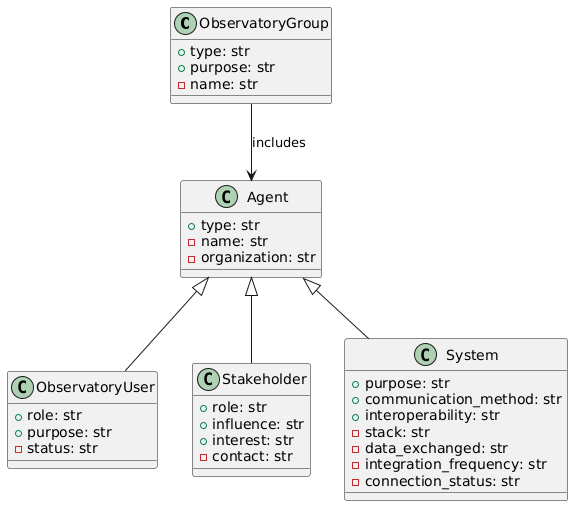
\includegraphics[width=1\linewidth]{imagens/mpo_agents_classification_tree.png}
    \caption{Árvore de classificação de conceitos da camada Agentes do MPO}
    \label{fig:mpo_class_tree}
\end{figure}

\section{Dicionário de verbos e Tabela de condições}

\begin{table}[H]
\centering
\caption{Dicionário de verbos da subcamada ``Gerenciar dados e informações`` da camada ``Processos``.}
\begin{tabularx}{\textwidth}{|l|X|X|X|}
\hline
\textbf{Verbo} & \textbf{Descrição} & \textbf{Agente} & \textbf{Objeto} \\ \hline
\textbf{Coletar} & Ação de obter dados e informações de fontes internas e externas relevantes aos projetos monitorados pelo observatório. & Observatório de projetos, usuário do observatório ou sistema externo & Dados brutos, informações de projetos ou indicadores preliminares. \\ \hline
\textbf{Tratar} & Ação de processar, limpar, padronizar e validar os dados coletados, garantindo consistência e integridade das informações. & Observatório de projetos, usuário do observatório ou sistema externo. & Dados coletados, metadados ou indicadores.\\ \hline
\textbf{Armazenar} & Ação de registrar e organizar os dados tratados em repositórios estruturados, permitindo sua recuperação e uso posterior. & Banco de dados do observatório & Dados tratados, conjuntos de indicadores ou séries históricas. \\ \hline
\textbf{Disponibilizar} & Ação de tornar os dados e informações acessíveis aos usuários do observatório, por meio de relatórios, painéis e serviços de consulta. & Observatório de projetos & Indicadores consolidados, relatórios, visualizações ou metadados públicos. \\ \hline
\end{tabularx}
\end{table}

\begin{table}[H]
\centering
\caption{Tabela de condições do verbo ``Coletar`` da subcamada ``Gerenciar dados e informações`` da camada ``Processos``.}
\begin{tabularx}{\textwidth}{|l|X|X|X|}
\hline
\textbf{Tipo} & \textbf{Condição} & \textbf{Resultado} \\ \hline
Pré-condição & As fontes de dados relevantes estão identificadas e acessíveis. &  O processo de coleta pode ser iniciado.\\ \hline
Pré-condição & O agente possui credenciais e permissões válidas para acessar as fontes de dados. &  A coleta ocorre de forma autorizada e rastreável.\\ \hline
Pós-condição & Dados brutos são capturados e registrados no sistema de coleta. &  Conjunto de dados brutos disponível para tratamento.\\ \hline
\end{tabularx}
\end{table}

\begin{table}[H]
\centering
\caption{Tabela de condições do verbo ``Tratar`` da subcamada ``Gerenciar dados e informações`` da camada ``Processos``.}
\begin{tabularx}{\textwidth}{|l|X|X|X|}
\hline
\textbf{Tipo} & \textbf{Condição} & \textbf{Resultado} \\ \hline
Pré-condição & Os dados coletados estão disponíveis e íntegros. & O sistema pode iniciar o processamento.\\ \hline
Pós-condição & São aplicadas regras de validação, limpeza e padronização. & Dados tratados e consistentes gerados.\\ \hline
Pós-condição & Dados inconsistentes são marcados e reportados para revisão. & Relatório de inconsistências armazenado.\\ \hline
\end{tabularx}
\end{table}

\begin{table}[H]
\centering
\caption{Tabela de condições do verbo ``Armazenar`` da subcamada ``Gerenciar dados e informações`` da camada ``Processos``.}
\begin{tabularx}{\textwidth}{|l|X|X|X|}
\hline
\textbf{Tipo} & \textbf{Condição} & \textbf{Resultado} \\ \hline
Pré-condição & Os dados tratados estão prontos e validados. & O armazenamento pode ser executado.\\ \hline
Pré-condição & O repositório de destino está disponível e possui espaço suficiente. & Inserção de dados é possível.\\ \hline
Pós-condição & Dados tratados são persistidos no banco de dados do observatório. & Conjunto de dados armazenado de forma estruturada e segura.\\ \hline
Pós-condição & Metadados associados são atualizados. & Sistema de armazenamento atualizado e pronto para consulta.\\ \hline
\end{tabularx}
\end{table}

\begin{table}[H]
\centering
\caption{Tabela de condições do verbo ``Disponibilizar`` da subcamada ``Gerenciar dados e informações`` da camada ``Processos``.}
\begin{tabularx}{\textwidth}{|l|X|X|X|}
\hline
\textbf{Tipo} & \textbf{Condição} & \textbf{Resultado} \\ \hline
Pré-condição & Os dados armazenados estão atualizados e validados. & Informações podem ser publicadas.\\ \hline
Pré-condição & O sistema de disseminação está operacional. & Publicação pode ocorrer.\\ \hline
Pós-condição & Dados e indicadores são apresentados em formato acessível (painéis, relatórios, APIs). & Usuários têm acesso aos dados de forma transparente e contextualizada.\\ \hline
Pós-condição & Acesso é registrado para auditoria e controle. & Histórico de disseminação atualizado.\\ \hline
\end{tabularx}
\end{table}

\begin{table}[H]
\centering
\caption{Dicionário de verbos da subcamada ``Produzir conhecimento e inteligência`` da camada ``Processos``.}
\begin{tabularx}{\textwidth}{|l|X|X|X|X|}
\hline
\textbf{Verbo} & \textbf{Descrição} & \textbf{Agente} & \textbf{Objeto} \\ \hline
\textbf{Transformar} & Ação de converter dados de um formato para outro. & Observatório de projetos ou usuário do observatório. & Dados tratados, conjunto de indicadores ou metadados.\\ \hline
\textbf{Classificar} & Ação de categorizar dados de acordo com critérios. & Observatório de projetos ou usuário do observatório. & Dados transformados ou conjunto de indicadores.\\ \hline
\textbf{Comunicar} & Ação de transmitir informações do observatório a públicos internos e externos. & Observatório de projetos ou usuários do observatório. & Relatórios, indicadores, boletins informativos, mensagens ou alertas.\\ \hline
\textbf{Visualizar} & Ação de exibir informações, permitindo ao usuário analisar os resultados. & Observatório de projetos. & Painéis de indicadores, Relatórios interativos, gráficos, tabelas ou mapas temáticos.\\ \hline
\textbf{Combinar} & Ação de integrar e relacionar dados oriundos de múltiplas fontes. & Observatório de projetos ou usuário do observatório. & Fontes de dados ou informações heterôgeneas.\\ \hline
\textbf{Refletir} & Ação de analisar os resultados do observatório, com o objetivo de extrair aprendizados. & Usuários do observatório. & Resultados dos projetos.\\ \hline
\textbf{Interagir} & Ação de estabelecer comunicação entre usuários, sistemas e componentes do observatório & Usuários do observatório. & Observatório de projetos.\\ \hline
\textbf{Acompanhar} & Ação de observar e registrar continuamente o andamento dos projetos e seus indicadores. & Usuários do observatório. & Projetos.\\ \hline
\textbf{Avaliar} & Ação de identificar sucessos, falhas e oportunidades de melhoria. & Usuários do observatório. & Projetos.\\ \hline
\textbf{Colaborar} & Ação de atuar com outros agentes para atingir objetivos em comum. & Usuários do observatório. & Observatório de projetos ou usuários do observatório. \\ \hline
\textbf{Responsabilizar} & Ação de atribuir responsabilidades a indivíduos envolvidos nos processos e resultados dos projetos. & Gestores do observatório. & Observatório de projetos.\\ \hline
\end{tabularx}
\end{table}

\begin{table}[H]
\centering
\caption{Tabela de condições do verbo ``Transformar`` da subcamada ```Produzir conhecimento e inteligência`` da camada ``Processos``.}
\begin{tabularx}{\textwidth}{|l|X|X|X|}
\hline
\textbf{Tipo} & \textbf{Condição} & \textbf{Resultado} \\ \hline
Pré-condição & Os dados de entrada foram tratados e validados. & A transformação pode ser iniciada com dados consistentes.\\ \hline
Pré-condição & As regras ou modelos de transformação estão definidos e acessíveis. & O processo de transformação pode ser configurado corretamente.\\ \hline
Pós-condição & Os dados foram convertidos para o formato de destino conforme o modelo de referência. & Dados transformados prontos para armazenamento ou disponibilização.\\ \hline
Pós-condição & O log de transformação foi gerado e armazenado para auditoria. & Histórico de transformações atualizado e rastreável.\\ \hline
\end{tabularx}
\end{table}

\begin{table}[H]
\centering
\caption{Tabela de condições do verbo ``Classificar`` da subcamada ```Produzir conhecimento e inteligência`` da camada ``Processos``.}
\begin{tabularx}{\textwidth}{|l|X|X|X|}
\hline
\textbf{Tipo} & \textbf{Condição} & \textbf{Resultado} \\ \hline
Pré-condição & Os dados ou projetos a serem classificados estão disponíveis e padronizados. & O processo de classificação pode ser executado de forma consistente.\\ \hline
Pré-condição & Os critérios, regras ou taxonomias de classificação estão definidos e atualizados. & O sistema pode aplicar corretamente as categorias correspondentes.\\ \hline
Pós-condição & Cada dado, informação ou projeto foi atribuído a uma ou mais categorias. & Conjunto de dados classificados disponível para análise e disseminação.\\ \hline
Pós-condição & As classificações foram registradas no banco de dados do observatório. & O sistema contém registros categorizados e rastreáveis.\\ \hline
\end{tabularx}
\end{table}

\begin{table}[H]
\centering
\caption{Tabela de condições do verbo ``Comunicar`` da subcamada ```Produzir conhecimento e inteligência`` da camada ``Processos``.}
\begin{tabularx}{\textwidth}{|l|X|X|X|}
\hline
\textbf{Tipo} & \textbf{Condição} & \textbf{Resultado} \\ \hline
Pré-condição & As informações ou resultados a serem comunicados estão validados e atualizados. & A comunicação pode ser iniciada com dados confiáveis.\\ \hline
Pré-condição & O canal de comunicação (portal, e-mail, boletim, API, etc.) está disponível e operacional. & O sistema pode executar a transmissão das informações.\\ \hline
Pós-condição & A mensagem, relatório ou indicador foi transmitido ao público-alvo. & O público recebeu a informação conforme planejado.\\ \hline
Pós-condição & O registro da comunicação foi armazenado para auditoria e acompanhamento. & Histórico de comunicações atualizado e rastreável.\\ \hline
Pós-condição & Feedback ou confirmação de recebimento foi registrado (quando aplicável). & Evidência de comunicação bem-sucedida armazenada.\\ \hline
\end{tabularx}
\end{table}

\begin{table}[H]
\centering
\caption{Tabela de condições do verbo ``Visualizar`` da subcamada ```Produzir conhecimento e inteligência`` da camada ``Processos``.}
\begin{tabularx}{\textwidth}{|l|X|X|X|}
\hline
\textbf{Tipo} & \textbf{Condição} & \textbf{Resultado} \\ \hline
Pré-condição & Os dados e indicadores estão atualizados e armazenados no sistema. & O módulo de visualização pode ser carregado com informações confiáveis.\\ \hline
Pré-condição & O usuário possui permissão de acesso à área ou tipo de dado solicitado. & A visualização é restrita ao nível de acesso autorizado.\\ \hline
Pós-condição & As informações são apresentadas em formato visual compreensível (gráficos, tabelas, mapas). & O usuário obtém uma visão clara e contextualizada dos dados.\\ \hline
Pós-condição & O sistema registra a sessão ou consulta realizada. & Histórico de visualizações atualizado para auditoria e métricas de uso.\\ \hline
Pós-condição & O usuário pode interagir com os dados (filtrar, comparar, detalhar). & Análise exploratória facilitada e experiência de uso aprimorada.\\ \hline
\end{tabularx}
\end{table}

\begin{table}[H]
\centering
\caption{Tabela de condições do verbo ``Combinar`` da subcamada ```Produzir conhecimento e inteligência`` da camada ``Processos``.}
\begin{tabularx}{\textwidth}{|l|X|X|X|}
\hline
\textbf{Tipo} & \textbf{Condição} & \textbf{Resultado} \\ \hline
Pré-condição & As fontes de dados a serem combinadas estão disponíveis e acessíveis. & O processo de integração pode ser iniciado.\\ \hline
Pré-condição & Os dados foram previamente tratados e padronizados em formatos compatíveis. & A combinação pode ocorrer sem perda de integridade.\\ \hline
Pós-condição & Os dados provenientes de diferentes fontes foram integrados com base em chaves ou atributos comuns. & Conjunto de dados combinado e consistente gerado.\\ \hline
Pós-condição & As regras de correspondência e fusão foram aplicadas corretamente. & Conjunto consolidado pronto para transformação ou análise.\\ \hline
Pós-condição & O registro do processo de combinação foi armazenado para rastreabilidade. & Log de integração disponível para auditoria e controle.\\ \hline
\end{tabularx}
\end{table}

\begin{table}[H]
\centering
\caption{Tabela de condições do verbo ``Refletir`` da subcamada ```Produzir conhecimento e inteligência`` da camada ``Processos``.}
\begin{tabularx}{\textwidth}{|l|X|X|X|}
\hline
\textbf{Tipo} & \textbf{Condição} & \textbf{Resultado} \\ \hline
Pré-condição & Os dados, indicadores e relatórios estão atualizados e acessíveis. & O processo de reflexão pode ser iniciado com base em informações válidas.\\ \hline
Pré-condição & O agente possui conhecimento do domínio e contexto institucional dos projetos analisados. & A reflexão será contextualizada e significativa.\\ \hline
Pós-condição & Foram identificados insights, tendências ou problemas a partir da análise das informações. & Conhecimento gerado para apoiar decisões estratégicas.\\ \hline
Pós-condição & As conclusões e recomendações foram registradas em relatórios ou atas. & <Resultados da reflexão documentados e compartilháveis.\\ \hline
Pós-condição & Sugestões de aprimoramento foram encaminhadas aos processos de planejamento ou decisão. & Ciclo de aprendizado institucional retroalimentado.\\ \hline
\end{tabularx}
\end{table}

\begin{table}[H]
\centering
\caption{Tabela de condições do verbo ``Interagir`` da subcamada ```Produzir conhecimento e inteligência`` da camada ``Processos``.}
\begin{tabularx}{\textwidth}{|l|X|X|X|}
\hline
\textbf{Tipo} & \textbf{Condição} & \textbf{Resultado} \\ \hline
Pré-condição & O usuário está autenticado e possui permissões adequadas para a interação. & A interação ocorre de forma segura e controlada.\\ \hline
Pré-condição & A interface de comunicação (portal, fórum, dashboard interativo, API etc.) está disponível e operacional. & A interação pode ser iniciada sem falhas técnicas.\\ \hline
Pós-condição & Uma troca de informações foi realizada entre o usuário e o sistema (ou entre usuários). & Comunicação ou colaboração efetivada.\\ \hline
Pós-condição & As interações foram registradas para auditoria e acompanhamento. & Histórico de interações atualizado e rastreável.\\ \hline
Pós-condição & O sistema respondeu ou atualizou informações em função da interação realizada. & Feedback processado e sistema atualizado conforme entrada do usuário.\\ \hline
\end{tabularx}
\end{table}

\begin{table}[H]
\centering
\caption{Tabela de condições do verbo ``Acompanhar`` da subcamada ```Produzir conhecimento e inteligência`` da camada ``Processos``.}
\begin{tabularx}{\textwidth}{|l|X|X|X|}
\hline
\textbf{Tipo} & \textbf{Condição} & \textbf{Resultado} \\ \hline
Pré-condição & Os projetos e seus indicadores estão cadastrados e atualizados no sistema. & O acompanhamento pode ser iniciado com informações válidas.\\ \hline
Pré-condição & O agente possui acesso autorizado aos dados de monitoramento. & O acompanhamento ocorre de forma segura e rastreável.\\ \hline
Pós-condição & O progresso dos projetos foi registrado e comparado com metas e prazos definidos. & O progresso dos projetos foi registrado e comparado com metas e prazos definidos. \\ \hline
Pós-condição & Foram identificadas variações ou desvios nos indicadores. & Alertas ou recomendações emitidos para ajuste de ações. \\ \hline
Pós-condição & As informações de acompanhamento foram integradas aos sistemas de análise e decisão. & Base de monitoramento consolidada e atualizada.\\ \hline
\end{tabularx}
\end{table}

\begin{table}[H]
\centering
\caption{Tabela de condições do verbo ``Avaliar`` da subcamada ```Produzir conhecimento e inteligência`` da camada ``Processos``.}
\begin{tabularx}{\textwidth}{|l|X|X|X|}
\hline
\textbf{Tipo} & \textbf{Condição} & \textbf{Resultado} \\ \hline
Pré-condição & Os dados de acompanhamento e desempenho dos projetos estão consolidados e validados. & A avaliação pode ser realizada com base em informações confiáveis.\\ \hline
Pré-condição & Existem critérios, indicadores e metas definidos para o processo avaliativo. & O julgamento de resultados segue parâmetros claros e comparáveis. \\ \hline
Pós-condição & O desempenho dos projetos foi analisado e classificado de acordo com os critérios estabelecidos. & Relatórios de avaliação elaborados e disponíveis para consulta.\\ \hline
Pós-condição & Foram identificados pontos fortes, fragilidades e lições aprendidas. & Geração de recomendações para aprimorar futuras iniciativas. \\ \hline
Pós-condição & As conclusões da avaliação foram comunicadas aos gestores e stakeholders. & Melhoria contínua e retroalimentação do ciclo de gestão do observatório.\\ \hline
\end{tabularx}
\end{table}

\begin{table}[H]
\centering
\caption{Tabela de condições do verbo ``Colaborar`` da subcamada ```Produzir conhecimento e inteligência`` da camada ``Processos``.}
\begin{tabularx}{\textwidth}{|l|X|X|X|}
\hline
\textbf{Tipo} & \textbf{Condição} & \textbf{Resultado} \\ \hline
Pré-condição & Os agentes envolvidos possuem acesso à plataforma de colaboração e estão cadastrados no sistema. & Os participantes podem iniciar interações colaborativas de forma autenticada.\\ \hline
Pré-condição & Há um projeto, tarefa ou objetivo compartilhado definido no ambiente do observatório. & A colaboração ocorre com propósito e foco claros.\\ \hline
Pós-condição & Foram registradas interações, contribuições e trocas de informações entre os agentes. & Histórico de colaboração documentado e disponível para análise.\\ \hline
Pós-condição & As contribuições coletivas resultaram em melhorias nos processos, produtos ou decisões do observatório. & Aprendizado organizacional e fortalecimento das redes de cooperação.\\ \hline
Pós-condição & As informações geradas na colaboração foram validadas e integradas aos repositórios do observatório. & Conhecimento colaborativo incorporado e acessível.\\ \hline
\end{tabularx}
\end{table}

\begin{table}[H]
\centering
\caption{Tabela de condições do verbo ``Responsabilizar`` da subcamada ```Produzir conhecimento e inteligência`` da camada ``Processos``.}
\begin{tabularx}{\textwidth}{|l|X|X|X|}
\hline
\textbf{Tipo} & \textbf{Condição} & \textbf{Resultado} \\ \hline
Pré-condição & Existem papéis, responsabilidades e normas institucionais claramente definidos no observatório. & O agente pode identificar e associar responsabilidades de forma legítima.\\ \hline
Pré-condição & Há registros de ações, decisões e resultados vinculados a agentes identificáveis. & A responsabilização pode ser fundamentada em evidências verificáveis.\\ \hline
Pós-condição & As responsabilidades foram formalmente atribuídas aos respectivos agentes. & Papéis e deveres institucionalizados no sistema de governança.\\ \hline
Pós-condição & Foram identificadas conformidades e não conformidades nas execuções dos projetos. & Ações corretivas ou sanções podem ser aplicadas conforme as normas.\\ \hline
Pós-condição & O processo de responsabilização foi documentado e disponibilizado para auditoria ou controle social. & Transparência e fortalecimento da accountability do observatório.\\ \hline
\end{tabularx}
\end{table}

\section{Tabelas de fórmulas}

\begin{table}[H]
\centering
\caption{Tabela de fórmulas do conceito "Serviços" da subcamada "Infraestrutura de TI" da camada "Estruturas".}
\begin{tabularx}{\textwidth}{|l|X|}
\hline
\textbf{Atributo} & \textbf{Fórmula} \\ \hline
\textbf{Provedor} & $\forall s \in Servico: s.Local \neq \emptyset$ \\ \hline
\textbf{Local} & $\forall s \in Servico: s.Local \neq \emptyset$ \\ \hline
\textbf{Período} & $\forall s \in Servico: s.Periodo.Início \leq s.Periodo.Fim$ \\ \hline
\textbf{Custo} & $\forall s \in Servico: s.Custo \geq 0$ \\ \hline
\textbf{Disponibilidade} & $\forall s \in Servico: \ 90 \leq s.Disponibilidade \leq 100$ \\ \hline
\end{tabularx}
\end{table}

\begin{table}[H]
\centering
\caption{Tabela de fórmulas do conceito "Hardware" da subcamada "Infraestrutura de TI" da camada "Estruturas".}
\begin{tabularx}{\textwidth}{|l|X|}
\hline
\textbf{Atributo} & \textbf{Fórmula} \\ \hline
\textbf{Local} & $\forall h \in Hardware: h.Local \neq \emptyset$ \\ \hline
\textbf{Capacidade de processamento}  & $\forall h \in Hardware:\ h.CapacidadeProcessamento > 0$ \\ \hline
\textbf{Capacidade de armazenamento} & $\forall h \in Hardware:\ h.CapacidadeArmazenamento > 0$ \\ \hline
\end{tabularx}
\end{table}

\begin{table}[H]
\centering
\caption{Tabela de fórmulas do conceito "Redes" da subcamada "Infraestrutura de TI" da camada "Estruturas".}
\begin{tabularx}{\textwidth}{|l|X|}
\hline
\textbf{Atributo} & \textbf{Fórmula} \\ \hline
\textbf{Local}  & $\forall r \in Rede:\ r.Local \neq \emptyset$ \\ \hline
\textbf{Estado} & $\forall r \in Rede:\ r.Estado \in \{Ativa, Inativa, EmManutencao\}$ \\ \hline
\textbf{Banda} & 
\parbox[t]{0.8\linewidth}{
A largura de banda mínima depende da quantidade de usuários concorrentes, do número médio de requisições por usuário por segundo, do tamanho médio das requisições e de um fator de segurança.  
Fórmula: 
\[
r.Banda \ge \frac{U \times R \times T \times 8}{1000} \times F
\]  
onde: 
U = usuários concorrentes,  
R = requisições por usuário por segundo,  
T = tamanho médio da requisição (KB),  
F = fator de segurança (ex.: 1,5–2,0).  
Resultado em Mbps.
} \\ \hline
\textbf{Segurança} & $\forall r \in Rede:\ r.Seguranca \in \{\text{Alta, Média, Baixa}\}$ \\ \hline
\end{tabularx}
\end{table}

\begin{table}[H]
\centering
\caption{Tabela de fórmulas do conceito "Gerenciamento de dados" da subcamada "Infraestrutura de TI" da camada "Estruturas".}
\begin{tabularx}{\textwidth}{|l|X|}
\hline
\textbf{Atributo} & \textbf{Fórmula} \\ \hline
\textbf{Nome} & $\forall g \in GerenciamentoDeDados:\ g.Nome \neq \emptyset$ \\ \hline
\textbf{Versão} & $\forall g \in GerenciamentoDeDados:\ g.Versao \ge 1$ \\ \hline
\end{tabularx}
\end{table}

\begin{table}[H]
\centering
\caption{Tabela de fórmulas do conceito "Software" da subcamada "Infraestrutura de TI" da camada "Estruturas".}
\begin{tabularx}{\textwidth}{|l|X|}
\hline
\textbf{Atributo} & \textbf{Fórmula} \\ \hline
\textbf{Nome} & $\forall s \in Software:\ s.Nome \neq \emptyset$ \\ \hline
\textbf{Versão} & $\forall s \in Software:\ s.Versao \ge 1$ \\ \hline
\end{tabularx}
\end{table}

\begin{table}[H]
\centering
\caption{Tabela de fórmulas do conceito "Coleta" da subcamada "Componentes" da camada "Estruturas".}
\begin{tabularx}{\textwidth}{|l|X|}
\hline
\textbf{Atributo} & \textbf{Fórmula} \\ \hline
\textbf{Ferramenta} & $\forall c \in Coleta:\ c.Ferramenta \neq \emptyset$ \\ \hline
\textbf{Volume} & $\forall c \in Coleta:\ c.Volume \ge 0$ \\ \hline
\textbf{Qualidade} & $\forall c \in Coleta:\ c.Qualidade \in \{\text{Alta, Média, Baixa}\}$ \\ \hline
\end{tabularx}
\end{table}

\begin{table}[H]
\centering
\caption{Tabela de fórmulas do conceito "Processamento" da subcamada "Componentes" da camada "Estruturas".}
\begin{tabularx}{\textwidth}{|l|X|}
\hline
\textbf{Atributo} & \textbf{Fórmula} \\ \hline
\textbf{Ferramenta} & $\forall p \in Processamento:\ p.Ferramenta \neq \emptyset$ \\ \hline
\textbf{Volume} & $\forall p \in Processamento:\ p.Volume \ge 0$ \\ \hline
\textbf{Desempenho} & $\forall p \in Processamento:\ p.Desempenho \in \{\text{Alto, Médio, Baixo}\}$ \\ \hline
\textbf{Resultado} & $\forall p \in Processamento:\ p.Resultado \neq \emptyset$ \\ \hline
\end{tabularx}
\end{table}

\begin{table}[H]
\centering
\caption{Tabela de fórmulas do conceito "Armazenamento" da subcamada "Componentes" da camada "Estruturas".}
\begin{tabularx}{\textwidth}{|l|X|}
\hline
\textbf{Atributo} & \textbf{Fórmula} \\ \hline
\textbf{Local} & $\forall a \in Armazenamento:\ a.Local \neq \emptyset$ \\ \hline
\textbf{Capacidade} & $\forall a \in Armazenamento:\ a.Capacidade \ge 0$ \\ \hline
\end{tabularx}
\end{table}

\begin{table}[H]
\centering
\caption{Tabela de fórmulas do conceito "Disseminação" da subcamada "Componentes" da camada "Estruturas".}
\begin{tabularx}{\textwidth}{|l|X|}
\hline
\textbf{Atributo} & \textbf{Fórmula} \\ \hline
\textbf{Canal} & $\forall d \in Disseminacao:\ d.Canal \neq \emptyset$ \\ \hline
\textbf{Frequência} & $\forall d \in Disseminacao:\ d.Frequencia \ge 0$ \\ \hline
\textbf{Ferramenta} & $\forall d \in Disseminacao:\ d.Ferramenta \neq \emptyset$ \\ \hline
\textbf{Formato} & $\forall d \in Disseminacao:\ d.Formato \neq \emptyset$ \\ \hline
\textbf{Alcance} & $\forall d \in Disseminacao:\ d.Alcance \neq \emptyset$ \\ \hline
\end{tabularx}
\end{table}

\begin{table}[H]
\centering
\caption{Tabela de fórmulas do conceito "Relacionamento" da subcamada "Componentes" da camada "Estruturas".}
\begin{tabularx}{\textwidth}{|l|X|}
\hline
\textbf{Atributo} & \textbf{Fórmula} \\ \hline
\textbf{Canal} & $\forall r \in Relacionamento:\ r.Canal \neq \emptyset$ \\ \hline
\textbf{Frequência} & $\forall r \in Relacionamento:\ r.Frequencia \ge 0$ \\ \hline
\end{tabularx}
\end{table}

\begin{table}[H]
\centering
\caption{Tabela de fórmulas do conceito "Projetos" da subcamada "Conteúdos" da camada "Estruturas".}
\begin{tabularx}{\textwidth}{|l|X|}
\hline
\textbf{Atributo} & \textbf{Fórmula} \\ \hline
\textbf{Nome} & $\forall p \in Projetos:\ p.Nome \neq \emptyset$ \\ \hline
\textbf{Duração} & $\forall p \in Projetos:\ p.Duracao \ge 0$ \\ \hline
\textbf{Orçamento} & $\forall p \in Projetos:\ p.Orcamento \ge 0$ \\ \hline
\textbf{Descrição} & $\forall p \in Projetos:\ p.Descricao \neq \emptyset$ \\ \hline
\textbf{Responsável} & $\forall p \in Projetos:\ p.Responsavel \neq \emptyset$ \\ \hline
\textbf{Status} & $\forall p \in Projetos:\ p.Status \in \{\text{Em Planejamento, em Execução, Concluído, Cancelado}\}$ \\ \hline
\end{tabularx}
\end{table}

\begin{table}[H]
\centering
\caption{Tabela de fórmulas do conceito "Usuários" da subcamada "Conteúdos" da camada "Estruturas".}
\begin{tabularx}{\textwidth}{|l|X|}
\hline
\textbf{Atributo} & \textbf{Fórmula} \\ \hline
\textbf{Ação} & $\forall u \in Usuarios:\ u.Acao \neq \emptyset$ \\ \hline
\end{tabularx}
\end{table}

\begin{table}[H]
\centering
\caption{Tabela de fórmulas do conceito "Observatório" da subcamada "Conteúdos" da camada "Estruturas".}
\begin{tabularx}{\textwidth}{|l|X|}
\hline
\textbf{Atributo} & \textbf{Fórmula} \\ \hline
\textbf{Nome} & $\forall o \in Observatorio:\ o.Nome \neq \emptyset$ \\ \hline
\textbf{Instituição} & $\forall o \in Observatorio:\ o.Instituicao \neq \emptyset$ \\ \hline
\end{tabularx}
\end{table}

\begin{table}[H]
\centering
\caption{Tabela de fórmulas do conceito "Partes interessadas" da subcamada "Atores" da camada "Agentes".}
\begin{tabularx}{\textwidth}{|l|X|}
\hline
\textbf{Atributo} & \textbf{Fórmula} \\ \hline
\textbf{Nome} & $\forall p \in PartesInteressadas:\ p.Nome \neq \emptyset$ \\ \hline
\textbf{Organização} & $\forall p \in PartesInteressadas:\ p.Organizacao \neq \emptyset$ \\ \hline
\textbf{Contato} & $\forall p \in PartesInteressadas:\ p.Contato \neq \emptyset$ \\ \hline
\end{tabularx}
\end{table}

\begin{table}[H]
\centering
\caption{Tabela de fórmulas do conceito "Equipe do observatório" da subcamada "Atores" da camada "Agentes".}
\begin{tabularx}{\textwidth}{|l|X|}
\hline
\textbf{Atributo} & \textbf{Fórmula} \\ \hline
\textbf{Nome} & $\forall e \in EquipeObservatorio:\ e.Nome \neq \emptyset$ \\ \hline
\textbf{Membros} & $\forall e \in EquipeObservatorio:\ |e.Membros| \ge 1$ \\ \hline
\textbf{Responsável} & $\forall e \in EquipeObservatorio:\ e.Responsável \neq \emptyset$ \\ \hline
\end{tabularx}
\end{table}

\begin{table}[H]
\centering
\caption{Tabela de fórmulas do conceito "Usuários do observatório" da subcamada "Atores" da camada "Agentes".}
\begin{tabularx}{\textwidth}{|l|X|}
\hline
\textbf{Atributo} & \textbf{Fórmula} \\ \hline
\textbf{Nome} & $\forall u \in UsuariosObservatorio:\ u.Nome \neq \emptyset$ \\ \hline
\textbf{Organização} & $\forall u \in UsuariosObservatorio:\ u.Organização \neq \emptyset$ \\ \hline
\textbf{Status} & $\forall u \in UsuariosObservatorio:\ u.Status \in \{\text{Ativo, Inativo}\}$ \\ \hline
\end{tabularx}
\end{table}

\begin{table}[H]
\centering
\caption{Tabela de fórmulas do conceito "Sistemas" da subcamada "Atores" da camada "Agentes".}
\begin{tabularx}{\textwidth}{|l|X|}
\hline
\textbf{Atributo} & \textbf{Fórmula} \\ \hline
\textbf{Nome} & $\forall s \in Sistemas:\ s.Nome \neq \emptyset$ \\ \hline
\textbf{Organização} & $\forall s \in Sistemas:\ s.Organização \neq \emptyset$ \\ \hline
\textbf{Tecnologia} & $\forall s \in Sistemas:\ s.Tecnologia \neq \emptyset$ \\ \hline
\textbf{Tipo de dado trocado} & $\forall s \in Sistemas:\ s.TipoDadoTrocado \neq \emptyset$ \\ \hline
\textbf{Frequência de integracao} & $\forall s \in Sistemas:\ s.FrequênciaIntegração \ge 0$ \\ \hline
\textbf{Status de conexao} & $\forall s \in Sistemas:\ s.StatusConexao \in \{\text{Ativo, Inativo, Em manutencao}\}$ \\ \hline
\end{tabularx}
\end{table}



% ----------------------------------------------------------
\chapter{Artefatos gerados}
% ----------------------------------------------------------

\begin{itemize}
    \item \href{https://github.com/kvojps/onto-mpo}{Repositório github com os artefatos gerados nesta pesquisa;}
\end{itemize}

\end{apendicesenv}
